\documentclass[english]{report}

\usepackage{geometry}
\geometry{verbose,headsep=50pt}
\usepackage{babel}
\usepackage{natbib}
\bibliographystyle{plainnat}
%\setcitestyle{authoryear,open={(},close={)}}
\usepackage{fancyhdr}
\usepackage{graphicx}
\usepackage{wrapfig}
\usepackage{gensymb}
\usepackage{booktabs}
\usepackage{amssymb}
\usepackage{amsmath}


\usepackage{geometry}
\geometry{
	a4paper,
	total={210mm,297mm},
	left=15mm,
	right=15mm,
	top=30mm,
	bottom=20mm,
}


\usepackage{caption}
\graphicspath{ {./} }
\usepackage{titlesec}
 \newcommand{\HRule}{\rule{\linewidth}{0.5mm}}

\titleformat{\chapter}{\normalfont\huge}{\thechapter.}{24pt}{\huge\it}

%removes chapternumber%
\usepackage{setspace}
%\doublespacing
\pagestyle{fancy}
\usepackage[colorlinks=false,hidelinks]{hyperref}
\begin{document}

\begin{titlepage} \begin{center} 
		% Upper part of the page. The '~' is needed because \\ % only works if a paragraph has started. 

\includegraphics[width=0.3\textwidth]{./logo}~\\[1cm] \textsc{\LARGE University of Cape Town}\\[1.5cm] \textsc{\Large APG4001S Geodesy}\\[0.5cm] 
% Title 
\HRule \\[0.4cm] { \huge \bfseries Determination of Normal Correction to Levelled Heights \\[0.4cm] } \HRule \\[1.5cm]
% Author and supervisor
  \noindent \begin{minipage}[t]{0.4\textwidth} \begin{flushleft} \large \emph{Author:}\\ Craig \textsc{Ferguson} \end{flushleft} \end{minipage}
% 
  \begin{minipage}[t]{0.4\textwidth} \begin{flushright} \large \emph{Supervisor:} \\ Dr.~R \textsc{Govind} \end{flushright} \end{minipage} \vfill 
% Bottom of the page 
  {\large \today} \end{center} \end{titlepage}
\tableofcontents
%\listoffigures


%\pagebreak
\begingroup
\renewcommand{\cleardoublepage}{}
\renewcommand{\clearpage}{}
\chapter{Introduction}

\section{Purpose and Overview}
The broadcast ephemeris for GPS satellites is often used for lower accuracy surveys that can be conducted in real-time by receivers using the C/A or P- codes. Such surveys might include tacheometry surveys or for stake-out assistance. The navigation message contains predicted satellite positions which are transmitted from the satellite in real-time. Satellites tracking data obtained from monitor stations around the world is used by the Master Control Station to compute new parameters for the satellite orbits. These parameters are then transmitted back to the satellites and the navigation message is updated.

The precise ephemeris is post-calculated using a least squares adjustment of the actual tracking data. These are more accurate because they are based on actual tracking data and not predicted data. The precise positions can only be obtained in 14-17 hours in the case of Rapid, or in 13 days for the final orbit.

In this report, a broadcast ephemeris will be calculated using a broadcast ephemeris algorithm, this will be compared to the precise ephemeris over a period of 24 hours. The purpose is to investigate the reliability over time of a single navigation messages satellite positions.
\endgroup

%\pagebreak
\begingroup
\renewcommand{\cleardoublepage}{}
\renewcommand{\clearpage}{}
\chapter{Aims and Objectives}

\section{Overview}
\begin{itemize}
	\item Compute ECF cartesian coordinates of the satellite every 15 minsutes using the broadcast ephemeris algorithm.
	\item read in IGS precise ephemeris file for week 1854 for the satellite position.
	\item Compute the radial vector for both.
	\item Plot differences at each epoch and ascertain the interval for which the broadcast ephemeris is most accurate with respect to precise ephemeris.
	\item display the RMS of the radial differences.
\end{itemize}
\endgroup

%\pagebreak
\begingroup
\renewcommand{\cleardoublepage}{}
\renewcommand{\clearpage}{}
\chapter{Method}
\section {Preliminaries}
\subsection{Ellipsoid Radius}
The local ellipsoid radius is  calculated using the Cartesian coordinates or the geographic coordinates as follows:
\begin{equation} 
r(\varphi)= \sqrt{x^{2}+y^{2}+z^{2}} = a \sqrt{1-\dfrac{e^{2}(1-e^{2})\sin^{2}\varphi}{1-e^{2}sin^{2}\varphi}}
\end{equation}
$ e^{2} $ is the ellipsoidal first eccentricity. 
$ e=\dfrac{E}{a} $ where$  E=\sqrt{a^{2}-b^{2}} $. a and b are the semi-major and semi-minor axes respectively.
\subsection{Geocentric Coordinates}
Spherical harmonic models are formulated in geocentric  coordinates (the ellipsoidal coordinates). The longitude remains the same for both but the latitude for a given geographic coordinate location is converted to a geocentric location using the formula :
\begin{equation} 
(\varphi^{*})= 
\Big[  \big(  \dfrac{b}{a}  \big)^{2} tan \varphi \Big]
\end{equation}
\subsection{ Normal Gravity}
The normal gravity $ \gamma_{0}$ is a function of latitude is  calculated using:
\begin{equation} 
\gamma(\phi)= \gamma_{e}\dfrac{1+ksin^{2}\phi}{\sqrt{1-e^{2}sin^{2}\phi}}
\end{equation}
where $\phi  $ is the latitude of the point of interest.
the values of $ \gamma_{e},k \ and \ e^{2} $ are inserted as geometric constants gathered from the ellipsoid of choice, where $ \gamma_{e} $ is the normal gravity at the equator and $ e^{2} $ is the first eccentricity. $ k $ is given as a constant but can also be calculated $ k=\dfrac{b_{y_{b}}-a_{y_{a}}}{a_{y_{a}}} $.


\section{Legendre Polynomials and Functions}
Zonal Legendre functions of order 0 are called Legendre polynomials \cite{nicoPhysicalgeodesy}. They are polynomials in $ t =cos \theta $. 
The Legendre polynomials were calculated as follows...

Step 1 using Rodrigues Formula:
\begin{equation} 
P_{l}(t) = \dfrac{1}{2^{l}l!}\dfrac{d^{l}(t^{2}-1)^{l}}{dt^{l}}
\end{equation}
Step 2 using Ferrers Formula:
\begin{equation} 
P_{lm}(t) = (1-t^{2})^{m/2}\dfrac{d^{m}P_{l}(t)}{dt^{m}}
\end{equation}

\subsection{Fully Normalised associated Legendre Functions}
The abbreviations $ t=sin \varphi^{*} \ and \ u=cos\varphi^{*} $ are used below. The normalisation process applied to an associated Legendre function is as follows:
\begin{equation} 
\bar{P}_{n,m}(t) = \sqrt{(k(2n+1))\dfrac{(n-m)!}{(n+m)!}}P_{n,m}(t)
\end{equation}

\subsection{Recursive Formula}
$ P_{n,m}(t) $ can be calculated using recursive formulas as well:
\begin{equation} 
\begin{aligned}
P_{n+1,0}(t) & = (2n+1) t P_{n,0}(t) - nP_{n-1,0}(t) \\
P_{n,n}(t) & = (2n-1) u P_{n-1,n-1}(t) \\
P_{n,m}(t) & = P_{n-2,m}(t)+(2n-1)uP_{n-1,m-1}(t)
\end{aligned}
\end{equation}

The following starting values are required:
\begin{equation} 
\begin{aligned}
P_{0,0}(t) & = 1 \\
P_{1,0}(t) & = t \\
P_{1,1}(t) & = u \\
P_{2,0}(t) & = \frac{3}{2} t^{2} - \dfrac{1}{2}\\
P_{2,1}(t) & = 3ut \\
P_{2,2}(t) & = 3u^{2} 
\end{aligned}
\end{equation}


\section{(Calculate Geoid undulation N as a function of Longitude and Latitude)}
\begin{equation} 
N(\lambda,\varphi)=\dfrac{GM_{g}}{\gamma(\varphi)r(\varphi)}\sum\limits_{n=2}^\infty  \big( \dfrac{a_{g}}{r(\varphi)} \big) \sum\limits_{m=0}^n 
\Big[  \bar{C}_{n,m}cos(m\lambda) +  \bar{S}_{n,m}sin(m\lambda)   \Big] \bar{P}_{nm}(cos\varphi^{*})
\end{equation}
	
 $ \bar{C}_{n,m}$ and $ \bar{S}_{n,m}$ are the spherical harmonic coefficients of degree and order $ n$ , $ m$ respectively. The mass gravity constant $ GM_{\mathrm{g}}$ and the scale factor $ a_{\mathrm{g}}$ are from the geopotential model. $ \bar{P}_{n,m}(cos\bar{\varphi})$ fully normalized associated Legendre functions. The harmonics $ \bar{P}_{n,m}$ are evaluated at the geocentric latitude $ {\varphi}^{*}$, ( not at the geographical latitude) $ \varphi$. 



\endgroup

%\pagebreak
\begingroup
\renewcommand{\cleardoublepage}{}
\renewcommand{\clearpage}{}
\chapter{Results and Discussion}
\section{Results}

Figure: \ref{fig:1} shows the difference in radial distance along the y-axis in meters and the number of minutes in that day along the x axis. The small dot along the line y=0 shows the position of the satellite at the specific epoch. The first 6 pass-overs for satellite 21 are shown. It can be seen that each broadcast ephemeris is only within 2m precision for 240 mins (120 mins before and 120 mins after broadcast). After this time, a new ephemeris should be calculated. Figure \ref{fig:2} shows a zoomed in version with the same x and y axis values and units. It clearly represents the large increase in error that occurs after 120 minutes. 
\begin{figure}[h]
	\centering
	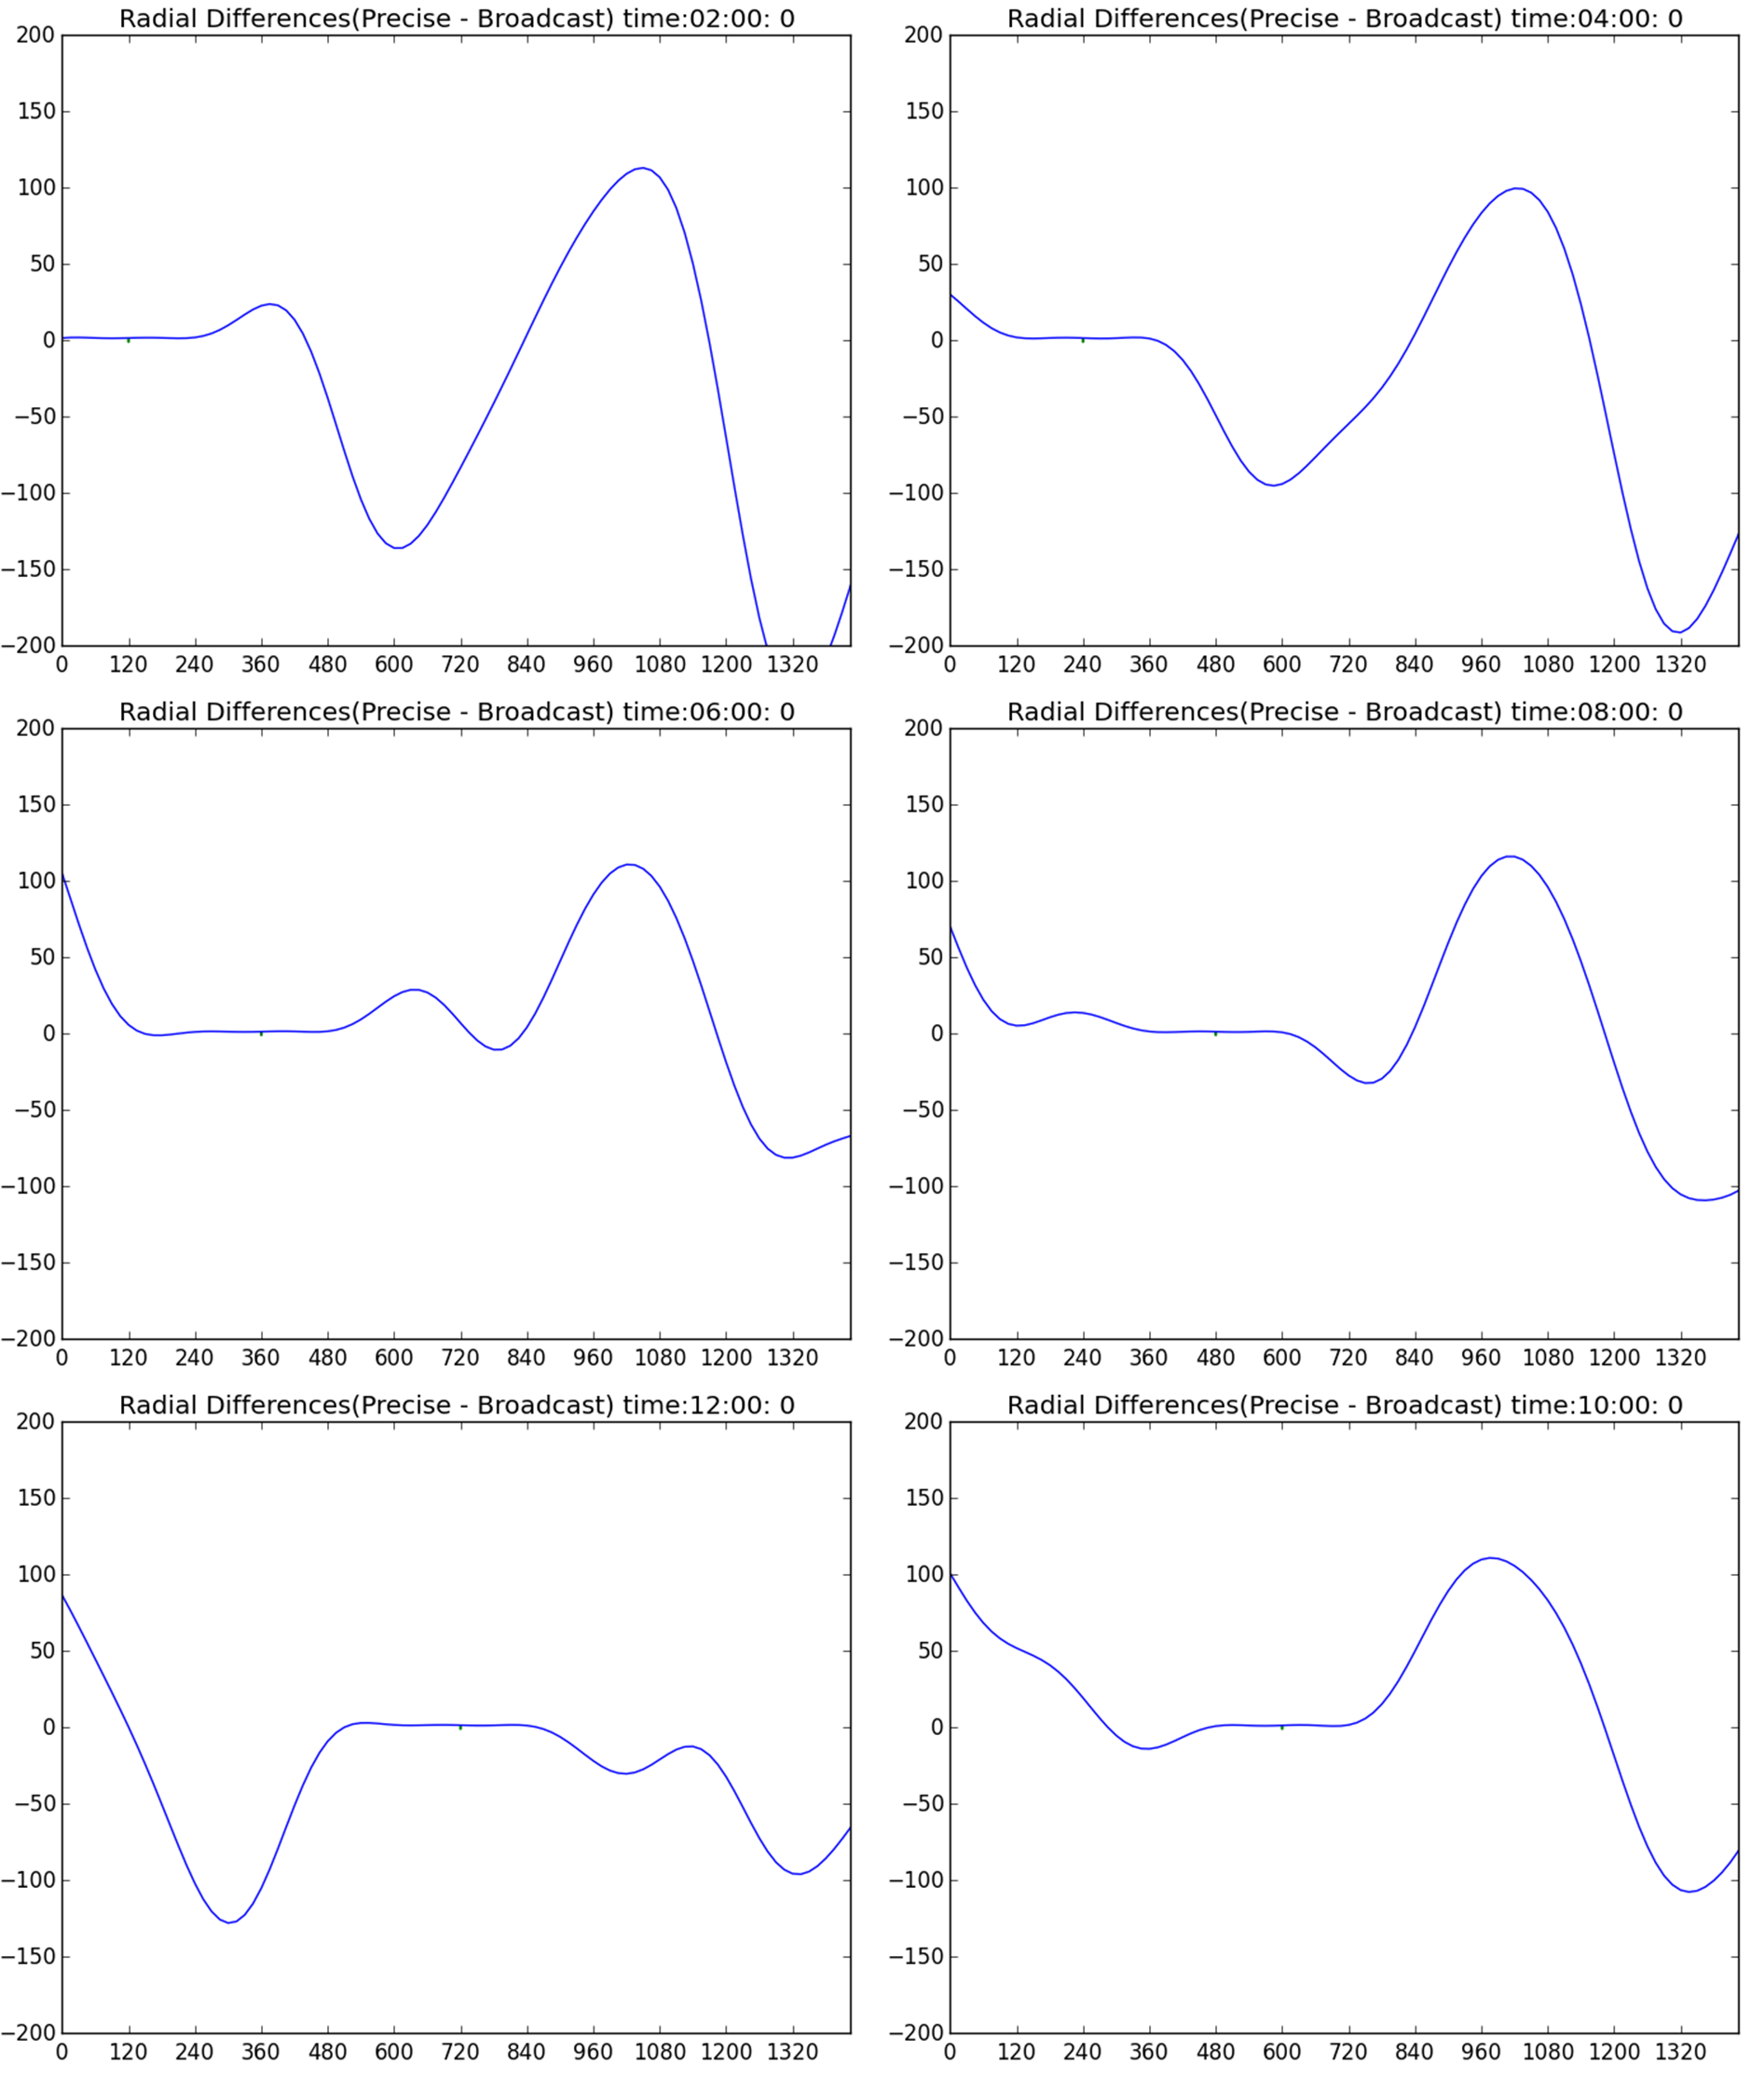
\includegraphics[width=0.6\textwidth]{r1.png}
	\caption{Various Times for Radial Differences}
	\label{fig:1}
\end{figure} 

\begin{figure}[h]
	\centering
	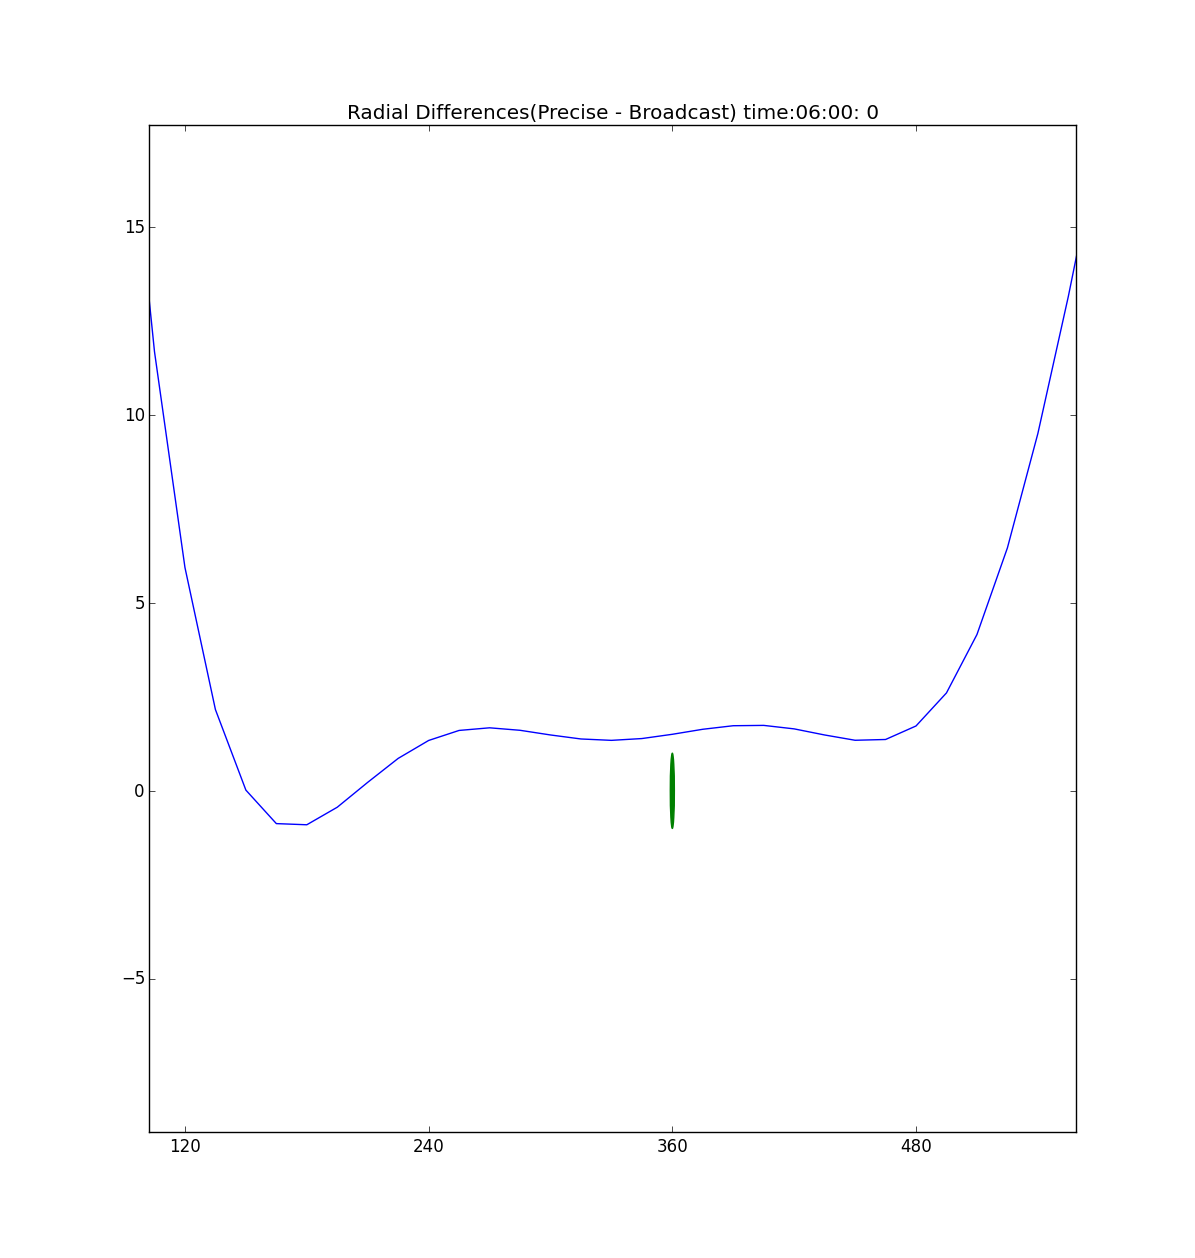
\includegraphics[width=0.6\textwidth]{6.png}
	\caption{Radial Differences (Precise - Broadcast) time-06h00}
	\label{fig:2}
\end{figure} 

% Table generated by Excel2LaTeX from sheet 'Sheet1'
\begin{table}[htbp]
  \centering
  \caption{Radial Differences at 15min Intervals at time t=06h00}
    \begin{tabular}{cccccr}
    \toprule
    88.66267 & 72.17792 & 56.48483 & \textbf{} & \textbf{} & \textbf{} \\
    \midrule
    29.83217 & 19.62730 & 11.69185 & \textbf{} & time  & \multicolumn{1}{c}{RMS (m)} \\
    2.16301 & 0.01845 & -0.87341 & \textbf{} &       &  \\
    -0.43708 & 0.22576 & 0.86294 & \textbf{} & 15mins & 1.41463 \\
    1.60730 & 1.67718 & 1.61113 & \textbf{} & 120mins & 1.49460 \\
    1.38003 & 1.34328 & \textbf{1.39116} & \textbf{} & 180mins & 2.08515 \\
    1.63826 & 1.73277 & 1.74156 & \textbf{} & 240mins & 5.81077 \\
    1.48629 & 1.34558 & 1.36609 & \textbf{} & 300mins & 16.05807 \\
    2.60659 & 4.15989 & 6.46676 & \textbf{} & \textbf{} & \textbf{} \\
    13.16141 & 17.15934 & 21.15208 & \textbf{} & \textbf{} & \textbf{} \\
    27.43905 & 28.91637 & 28.87017 & \textbf{} & \textbf{} & \textbf{} \\
    23.83664 & 19.11163 & 13.38262 & \textbf{} & \textbf{} & \textbf{} \\
    \bottomrule
    \end{tabular}%
  \label{tab:1}%
\end{table}%

\begin{figure}[h]
	\centering
	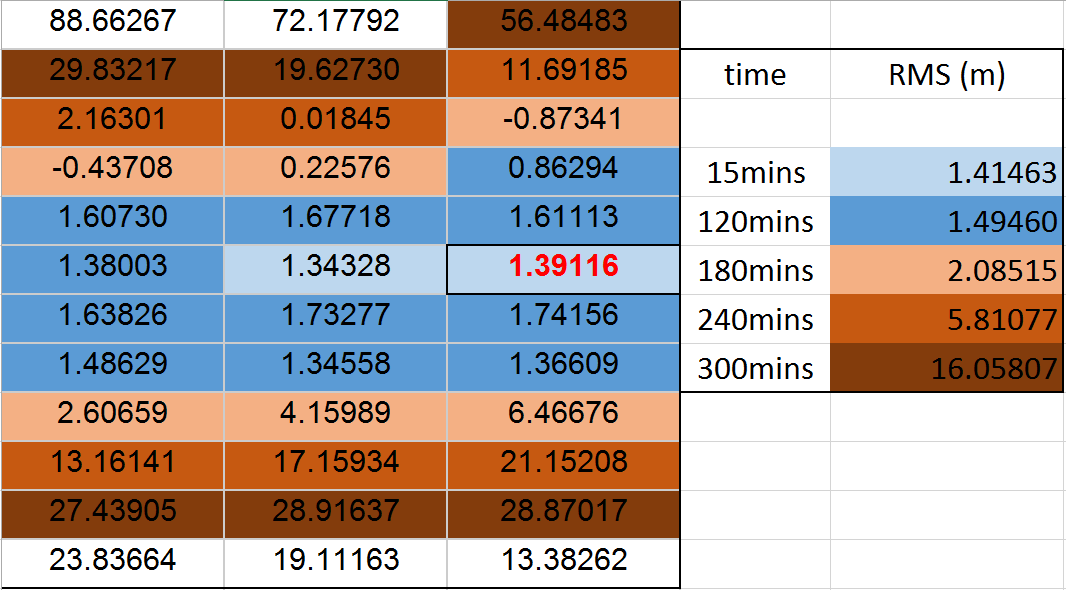
\includegraphics[width=0.8\textwidth]{rms.png}
	\caption{Radial Differences at 15min Intervals (Color Coded)}
	\label{fig:3}
\end{figure} 
The RMS calculations between ephemeris for the epoch 06:00:00 are shown in table \ref{tab:1} and figure \ref{fig:3}. Figure \ref{fig:3} is colour coded for improved visual interpretation.

The mins column show how much time before and after the navigation message. 
 It can be seen that there is not much improvement from 15 mins to 120 mins each side, but RMS rises above 2m after 180 minutes and continues to become unstable reaching over 16m after 5 hours.
\endgroup





\renewcommand{\bibname}{References}
\bibliography{references}

\end{document}
